\chapter{Notes}

\section{Book I}

\subsection{Statistics}
\begin{itemize}
	\item The GEV is not particularly useful for VaR estimation since VaR does not consider the distribution of maximum, but it is useful for stress testing.
	\item GPD is defined through a scale parameter $\beta \ge 0$ and tail shape parameter $\xi$, which can be any real number.
	\item Fat tails generate a positive GPD shape parameter, which indicates that VaR estimates are probably too small.
	\item POT approach requires a choice of a threshold, which may introduce additional uncertainty.
	\item POT approach serves as a basis for an expanded model of risk estimation.
	\begin{itemize}
		\item Under POT method, in the case of fat tails, not all moments are defined.
		\item POT is often estimated with a GPD.
	\end{itemize}
	\item The chi-square distribution is used to test how closely the selected distribution fits the actual data.
\end{itemize}
\subsection{VaR and ES}
\begin{itemize}
	\item The major improvement of the non-parametric approach over the traditional historical simulation approach is that VaR can be calculated for a continuum of points in the data set.
	\item Assuming normal distribution, both VaR and ES satisfy all properties of coherent risk measure. Assuming non-normal distribution, only ES satisfies the requirements.
	\item VaR is the most widely used risk measure for both capital allocation and absolute risk calculation purposes. However, ES is increasingly being used for capital allocation purposes.
	\item When backtesting VaR Error Type I is "rejecting correct model" and Error Type II is "accepting incorrect model". 
	Regulators are more affraid of Error Type II and of Error Type I.
	\item Economic capital models are quite similar to VaR models despite the longer time horizons, higher confidence levels, and greater lack of data.
\end{itemize}

\subsection{Interest Rate Models}
\begin{itemize}
	\item Basis point volatility of CIR model increases at rate $\sigma \sqrt{r}$, while log-normal basis-point volatility increases at rate $\sigma r$. Thus CIR basis-point volatility is less than log-normal basis point volatility.
\end{itemize}

\subsection{Fixed Income Valuation and Options}
\begin{itemize}
	\item Position-based risk measures evaluate the manager's holdings on a current basis and can thus detect style drift more quickly. Return-based risk measures evalute risk using historical returns and are therefore not convenient for style drift detection.
	\item LIBOR is commonly used as a risk-free rate for non-collateralised transactions.
	\item Local valuation methods measure portfolio risk by valuing assets at one point in time, then making adjustments to relevant risk factors that are expected to cause changes in the overall portfolio value. The delta-normal valuation is an example of a local method.
	\item The assumption that the relationship between an option's price and the ratio of the underlying to strike price applies in subsequent periods is known as sticky-delta rule. The assumption that an option implied volatility is the same over a short period of time is called the sticky-strike rule.
	\item When put feature expires on a bond (so that it becomes option-free), the curve depicting the price and yield relationship of the bond becomes less convex.
\end{itemize}

\section{Book II}

\subsection{Credit Risk Models}
\begin{itemize}
	\item Under Merton model, value of a firm at maturity of the ZCB is defined as $max(A_T - D, 0)$.
	\item Under Merton model the option on equity is a call-on-call compound option and cannot be valued using the Black-Scholes-Merton option pricing model (Geske model is used instead).
	\item KMV model is most sensitive to asset return volatility and asset return correlation estimates. It employs equity price volatility as a proxy for asset price volatility.
	\item In CreditRisk+ model, the bankruptcy / recovery process are exogenous. It only focuses on default events and ignores prices, spreads, and mitigations. It measures the credit risk of a portfolio using a set of common risk factors for each obligor. The model assumes that the defaults are uncorrelated across obligors.
	\item CreditMetrics calculates the change in portfolio value due to credit migration of the underlying bonds.
	\item Shimko, Tejima and van Deverter (1993) model states
	\begin{itemize}
		\item interest rate volatility increase $\rightarrow$ lower value of debt
		\item higher correlation between firm values and changes in interest rates $\rightarrow$ lower value of debt
		\item higher value of speed term $\rightarrow$ lower value of debt
	\end{itemize}
	\item Neymann-Pearson rule minimises type I error (lending to a risky company) with type II error (not lending to a non-risky company) remaining constant.
\end{itemize}

\subsection{Securitized Instruments and Credit Derivatives}
\begin{itemize}
	\item A downgrade by a bond-rating agency is not used  as a trigger for payments on a default swap. The reason is that downgrades are often rare and using them might harm independence of a rating agency.
	\item Invocation of cross-default clause is a credit event.
	\item CDS will provide a hedge with regard to operations risk, provided that the operational problem is serious enough.
	\item A digital CDS will pay off a pre-determined fixed amount in the event of a default. Digital CDS is often used against highly illiquid reference assets that would be difficult to price.
	\item CLN issuer has no counterparty risk.
	\item Originator / manager of a securitization would most likely bear the first loss in the capital structure in order to help align their interest with investors and minimise conflicts of interest in order to make the security less risky.
	\item A collateral loan obligation (CLO) is a specialised form of CDO that only invests in bank loans.
	\item Government securities are the least likely used as collateral for CDO, since CDOs are constructed to give access to certain risk / return opportunities. Bonds, loans and mortgages are used individually or collectively to collateralized CDOs.
	\item All early prepayments within a lock-out period are reinvested into new loans. After lock-out period the prepayments are used to amortise the highest tranches.
	\item When securitizing pool of credits, at least one tranche has an investment grade (even if the underlying credits have rating of B or CCC).
	\item In case of CDO, SPV is typically AAA rated.
	\item When calculating default sensitivities of equity, mezzanine and senior tranches, various hypothetical default probabilities (not a CDS curve!) are shocked. Default sensitivities are the largest at values that create losses close to the attachment points.
	\item The two trust structure allows the assets conveyed to be sufficiently distanced from the originator. Thus the assets are considered a true sale and the trust is bankruptcy remote.
	\item Assets have to be transferred from the loan originator to the SPV through a "true sale" for a securitization to have transferred real ownership of the assets.
	\item Ring fencing is undertaken to provide a higher credit rating to a subsidiary than is available to the parent. Derivative products companies or unregulated subsidiaries of investment banks are examples of such structures. Aim is to create a structure that is bankruptcy remove from its parent. 
	\item The behaviour of default sensitivities for tranches are most similar to high gammas for at-the-money options. Default sensitivities are always positive and are the largest when the resulting loss is close to the attachment point.
	\item Mortgage-back securities exhibit negative convexity - their NPV declines more when interest rates rise then it increases when interest rates fall. Standard bond / loan exhibits positive convexity.
\end{itemize}

\subsection{Counterparty Risk, Collateral Management and Central Counterparty}
\begin{itemize}
	\item Banker's paradox is associated with a break clause (also called a liquidity put or early termination option).
	\item A swap paying the higher interest rate has a greater exposure than swap paying lower interest rate due to the fact that it has a significantly higher gain on the notional value at the maturity of both swaps. In addition, over the long term, the interest reate drift dominates the implied volatility measure. This causes the PFE for the swap receiving the higher interest rate to remain relatively flat.
	\item ISDA master agreements lower transaction costs because of their operation efficiency.
	\item Collateralization should be viewed as proposition to, but not a replacement for, ongoing due diligence review of credit quality and exposures. Collateralization may improve asset recovery in the event of default, give rise to additional risks, and can be viewed as a "double-edge" sword.
	\item Under the limited two-way payment covenant clause, the non-defaulting counterparty is not required to pay if the final net amount is favourable to the defaulting party.
	\item Legal risk, documentation risk and liquidity risk are residual risks that may arise when credit risk mitigation techniques are applied. Therefore, inability to secure collateral would be a residual risk.
	\item Contract is (a) bilateral with counterparty risk or (b) unilateral with lending risk.
	\item With an unfunded bilateral contract, both parties take on risk. As such, a trade on the OTC market would be a bilateral contract and carry counterparty risk. Bank loans and exchange traded options are unilateral contracts as only one party takes on risk.
	\item Traditionally, when quantifying credit exposure, there is an assumption of zero recovery value.
	\item \textit{running spread CVA  = EPE(\%) * credit spread (\%)}
	\item Assumptions to approximate CVA as a running spread include
	\begin{itemize}
		\item EPE and PD are constant,
		\item EE or PD are symmetric
	\end{itemize}
	\item CVA falls to zero in the case of default.
	\item In case of counterparties with which bank has other credit exposure, only facility LGD (= LGD for the specific OTC derivative) needs to be calculated (PD is facility independent).
	\item Only some (not all) central counterparties (CCP) are too important to fail (TIFF).
	\item General clearing members (GCMs), individual clearing members (ICMs) and non-clearing members (NCMs) can all trade through a central counterparty.
	\item A bank run is the most common example of systemic risk.
	\item Multilateral netting requires knowledge of the positions of all members. However, institutions may wish to keep the information secret. As a result, disclosure is one of the disadvantages of multilateral netting.
	\item Credit exposure is defined both for pricing and risk management wheres VaR is defined only for risk management.
	\item A credit spread based on a single liquid observation can be used as an alternative to a credit spread curve based on multiple issues and maturities. The credit spread is estimated from a single observation and is added to the reference curve at a constant rate of percentage.
	\item Upward-sloping spread curves generate cumulative default 
	distributions that are flatter in the short-term but steeper afterwards. Downward-slopping spread curves are steeper in the short-term as the near probability of default is higher but then moderates to flatter curve afterwards.
	\item Specific risk exposure refers to securities that undergo adverse price movements as a result of idiosyncratic factors related to individual issuers. Thus, government debt issues and futures contracts based on diversified indices (e.g. S\&P 500) are not exposed to specific risk.
	\item Correlation risk applies to market risk, credit risk, systemic risk and concentration risk as well.
\end{itemize}

\subsection{Mortgages}
\begin{itemize}
	\item Sub-prime market is characterised by high debt service ratios of 50\% or higher.
	\item For sub-prime hybrid loans are typically of 2/28 or 3/27 schemes where only the first 2Y or 3Y are fixed. The bank reduces its exposure to a floating rate inflow (asset) by entering into pay-floating / receive fixed swap.
	\item Score cards
	\begin{itemize}
		\item behaviour score - assess existing customer credit usage and historical delinquencies
		\item revenue score - evaluate existing customers on potential profitability
		\item response score - assign a probability to whether a customer is likely to respond to an offer
		\item attrition score - probability of reduction or elimination of outstanding debt by existing customer
	\end{itemize}
	\item A FICO score of 660 or above is considered by most credit scoring firms as a prime credit.
	\item A charge-off is declaration by creditor (usually a credit card company) that an amount of debt is unlikely to be collected.
	\item Deliquency ratio is calculated as $\frac{\textit{credit cards 
	receivables over 90D}}{\textit{total credit card pool}}$.
\end{itemize}

\section{Book III}

\subsection{Basel and Capital Requirements}
\begin{itemize}
	\item capital requirements - CRE $>$ OPR $>$ ALM
	\item Since Basel II parameters are calibrated on G-7 banks, they tend to underestimate the risk at emerging market banks.
	\item Within the banking industry, systemic risk is more of an issue, thus the stability of the overall financial system is more of a focus within Basel II / III. In contrast, Solvency II focuses more on the individual policyholders.
	\item The following six risk types are all related to underwritting risk within the insurance sector - life and health, non-life, market, counterparty default, operational, and intangibles.
	\item Tier 1 capital (also called core capital) is composed of common equity, non-cumulative perpetual preferred stocks, and minority equity interest in consolidated subsidiaries, less goodwill and other deductions.
	\item Tier 2 capital (also called supplementary capital) is composed of hybrid instruments that are structured to be more or less permanent. These include perpetual shares, subordinated debt of initial maturity of not less than 5Y and quality 99Y debt. Tier 2 capital also includes unrealised gains on long term investments.
	\item Under Basel II, Tier 2 capital must be lower or equal to Tier 1 capital. This implies that \textit{total 
	capital = Tier 1 + min(Tier 1, Tier2) - deductions}.
	\item For Basel III purposes, the leverage ratio is Tier 1 capital / total exposure.
	\item For operational risk under Basel II there can be within-cell dependencies which include both frequency and severity dependencies.
	\item When modelling LDA, extrapolation of observed losses, in order to develop a more complete severity distribution of losses, could result in overestimation of the needed capital charge due to "including" severe hypothetical losses.
	\item Under Basel II securitized positions rated below BB- / unrated are subject to deductions. A deduction implies that capital equivalents to the securitization tranche must be hold. Deductions are excluded only for estimating capital change for market risk.
	\item Revision to Basel II market risk framework requires banks to establish and uphold procedures for computing adjustments to the current value of liquid securities. The adjustment is made regardless of which of the positions is market to market, market to model or obtained through third-party valuation. When determining accuracy and sensibility of adjustment, the following factors are taken into account
	\begin{itemize}
		\item market concentration,
		\item average volatility of bid-ask spread,
		\item average trading volume and
		\item age of the position
	\end{itemize}
	\item Under Basel II market risk include
	\begin{itemize}
		\item equities
		\item interest rates
		\item foreign exchange
		\item commodities (single factor model is sufficient for institutions with limited or aggregated positions)
		\item options
	\end{itemize}
	\item Under IRB approach to the credit risk first loss piece (equity tranche) must be fully deducted from regulatory capital.
	\item To compute regulatory capital under IRB approach for securitization exposures under the Basel II framework, the following can be used
	\begin{itemize}
		\item rating based approach - must be used if external rating is available
		\item internal assessment approach
		\item supervisory formula
	\end{itemize}
	\item Both Internal Assessment Approach (IAA) and Supervisory Formula (SF) approach could be used for unrated securitized assets. IAA is only used in limited situations, with specific permission from the regulatory authority. IAA is based on methodology used by external rating agencies.
	\item Under Pillar II, regulator must assess impact of interest rate risk on bank's capital position through a +200bps shock.
	\item The purpose for addressing market discipline in Basel II is to benefit market participants, banks, investors and regulators of timely and relevant banking operations and activities while simultaneously recognising the sensitivity of proprietary internal operations.
	\item Under IRB approach, calculation of weights should be independent of specific portfolio. This so-called portfolio invariance referes to the fact that risk weights do not explicitly incorporate correlations among assets within the portfolio.
	\item Basel II risk weight function for IRB is based on ASRF model, under which the system-wide risks that affect all 
	obligors are modelled with only one systematic risk factor. The major reason for using ASRF is that the model should be portfolio invariant, so that the capital required for any given loan depends only on the risk of that loan and does not depend on the portfolio it is added to.
	\item With respect to including insurance, an analyst is allowed to reduce the severity of losses that exceed a given deductible but she cannot adjust the frequency.
	\item Capital requirements under IRB approach increase concavely with PD and linearly with LGD. With increasing PD, capital requirements are increasing at a decreasing rate due to decreasing correlations.
	\item Under advanced IRB, banks are allowed to provide their own estimates of PD, LGD and EAD, but must use correlation coefficient formula provided by the supervisor.
	\item When adopting IRB method, a voluntarily return to standard approach is not permitted.
	\item When estimating credit portfolio losses, LGD is not a critical parameter to estimate. PD and default correlations are of much higher importance.
	\item Under Basel II, banks cannot use external rating for some counterparites and internal ratings for other. The reason is to avoid "cherry picking".
	\item HQLA assets received through rehypothecation can be included in the stock of HQLA if they cannot be withdrawn during a stress period by owner.
	\item In contrast to credit risk IRB approach, banks using AMA may have to set aside capital for both expected and unexpected operational loss.
\end{itemize}

\begin{figure}[htp]
\centering
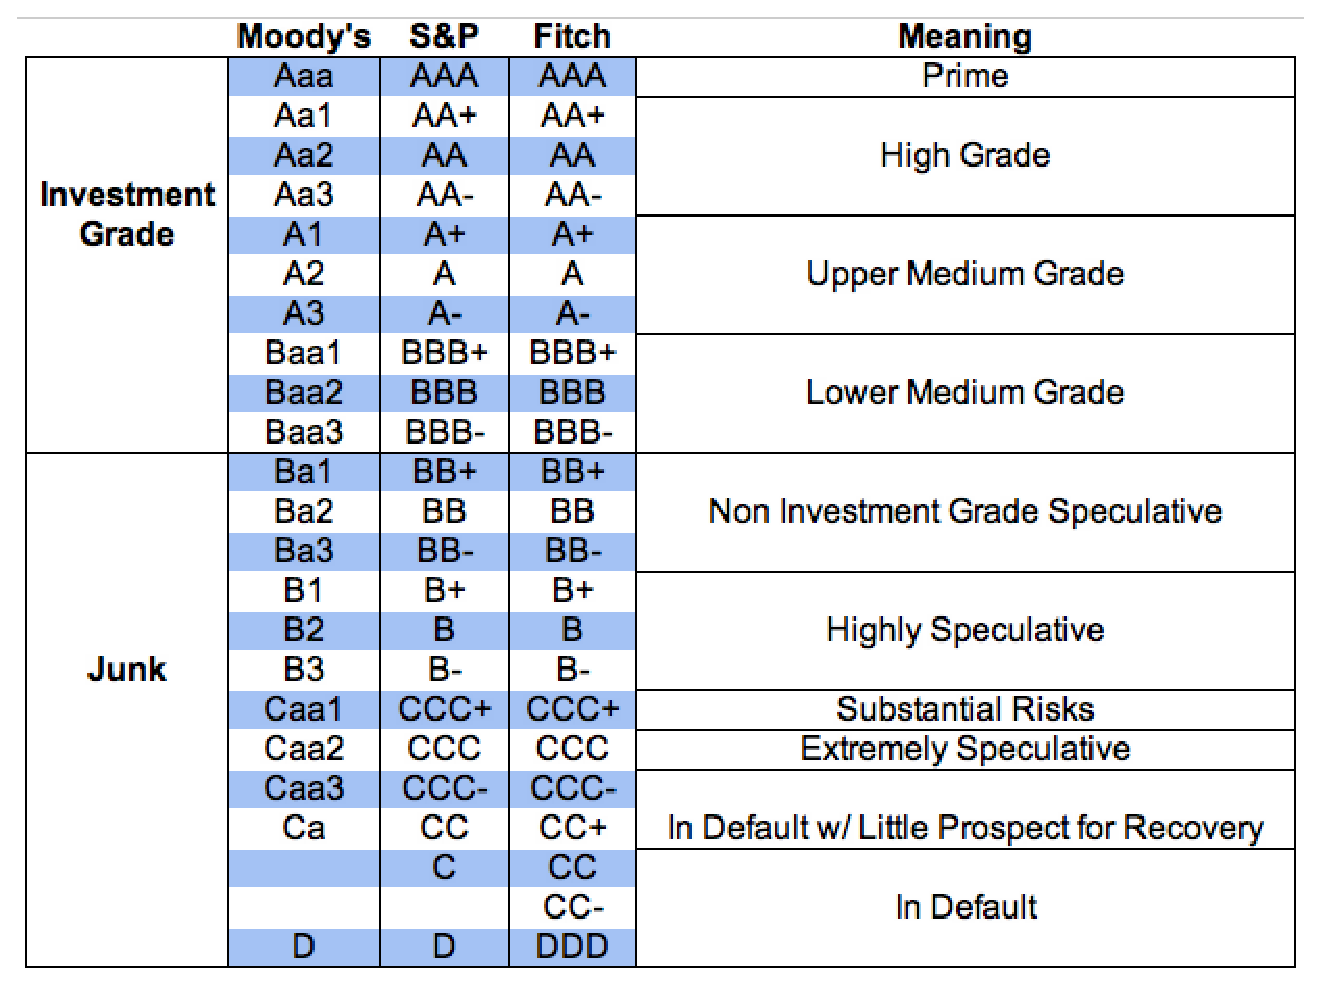
\includegraphics[scale = 0.50]{credit_ratings.eps}
\caption{Credit ratings}
\label{credit_ratings}
\end{figure}

\subsection{Model Risk}
\begin{itemize}
	\item model risks
	\begin{itemize}
		\item incorrect implementation - model is correctly specified and calibrated but incorrectly implemented
		\item incorrect calibration - inaccurate / infrequent calibration
		\item incorrect model application - e.g. low number of Monte-Carlo simulations
	\end{itemize}
	\item Models should be judged on their predictive ability rather than on their assumptions.
	\item At institutional level, the goal of model risk management is to reduce the likelihood that recorded values and future observed market values will differ.
	\item Basis risk arises when a position or its hedge is mapped to the same set of risk factors, which can be done when it is difficult to distinguish between two closely related positions.
	\item In early 2012, JP Morgan informed its regulator Office of the Controller (OCC) that the new VaR model cut bank's VaR by 50\%. The OCC failed to inquire about the dramatic drop in risk, the efficiency of the new model, or reasons for the change. The OCC never concluded that the new VaR model failed to properly reflect risks.
\end{itemize}

\subsection{Liquidity Risk}
\begin{itemize}
	\item Liquidity risk is the degree to which a trader cannot trade a position without excess cost, excess risk, or inconvenience.
	\item Trade processing costs are typically not a substantial component of liquidity risk.
	\item For endogenous markets, if a trader attempts to liquidate (buy) a large position, the trader should expect the bid (ask) price to fall (increase) and bid-ask spread to widen.
	\item ABCD does not have an active secondary market and has significant liquidity risk. ABCP pools assets from multiple issuers and continually purchases new assets and offers new issues.
\end{itemize}

\section{Book IV}

\subsection{Portfolio Management}
\begin{itemize}
	\item Screening technique strives for risk control by including a sufficient number of stocks that meet the screening parameters and by weighting them to avoid concentration in any particular stock.
	\item Linear programming builds on stratification technique. It does not necessarily select the portfolio with the lowest level of active risk. Rather, linear programming attempts to improve stratification by introducing many more dimensions of risk control and ensuring that the portfolio approximates the benchmark for all these dimensions.
	\item Quadratic programming allows for risk control through parameter estimations but generally requires many more inputs estimated from market data than other method requires because it entails estimating volatilities and pair-wise correlations between all assets in a portfolio. Quadratic programming is a powerful process, but given the large number of inputs it introduces the potential for noise and poor calibration.
\end{itemize}

\subsection{Hedge Funds}
\begin{itemize}
	\item Hedge fund assets grew to 1.4 trillion USD by 2007.
	\item During the 2001 - 2010 time period, all three hedge fund databases substantionally outperformed equities, accompanied by less than half the standard deviation of equities.
	\item For investment funds historical performance review is not part of an operational due diligence questionnaire. It is reviewed separately.
	\item For investment funds
	\begin{itemize}
		\item business model risk can be assessed by considering revenues and expenses, sufficiency of working capital, existence of budgets, computation of break-even points, ability to increase investment asset base, existence of key person insurance and existence of a succession plan,
		\item fraud risk can be assessed by considering the existence of related-party transactions, liquidity, litigation, unreasonably high (stated) investment returns, personal trading by the manager of the same or similar securities as those held by the fund and shorting transactions.
	\end{itemize}
	\item Typical long / short hedge strategy would target net long position.
	\item Merger arbitrage hedge funds are exposed to the event risk of a collapsed merger deal. Thus, the fund is exposed to large downside risk that is similar to credit risk.
	\item Managed futures hedge funds may help mitigate risk associated with a market wide funding crisis due to their convex performace profile.
	\item After a hedge fund is closed, the historical data of the fund is seldom included in data for future analysis. The reasons are (a) investors desire the analysis of funds that are investable and (b) funds that are shut down do not wish to disclose data for legal reasons. This effect is called survivorship bias.
	\item A higher level or risk aversion and lower transaction costs lead to lower dispersion risk.
	\item When testing Jensen $\alpha$ we use t-statistics in form of $t = \frac{\alpha}{\sigma_{\alpha}}$ or $t = \frac{\alpha}{\sigma / \sqrt{N}}$.
	\item When calculating a hurdle rate to be compared with RAROC, weights of equity are based on market rather than on book value.
\end{itemize}

\subsection{Pension Risk}
\begin{itemize}
	\item From the plan sponsor's perspective nominal pension obligations are similar to a short position in a long-term bond. Therefore nominal pension obligations are similar to a short position in a bond.
	\item In case of a pension fund a mismatch between asset and liability value is called a funding risk.
\end{itemize}

\subsection{Other}
\begin{itemize}
	\item The same individual or team responsible for identifying and clasifying the firm's information assets should 
	be also responsible for assessing those assets and managing and reporting the risk. 
	\item Stress scenarios do not typically incorporate the possibility that traders will re-hedge positions during times of market shocks.
\end{itemize}



